\documentclass{beamer}
\usepackage[utf8]{inputenc}

\title{Jee linalg 2d Problem 35}
\author{EE17BTECH11017  EE17BTECH11020}
\date{}
\begin{document}
\frame{\titlepage}

\begin{frame}
\frametitle{Geometry Question}
A straight line through the origin \textbf O meets the lines
\\4\textbf x + 3\textbf y = 10
\\8\textbf x + 6\textbf y + 5 = 0
\\at \textbf A and \textbf B respectively. Find the ratio in which \textbf O divides \textbf{AB}.
\end{frame}

\begin{frame}
\frametitle{Matrix transformation of the question}
A straight line through the origin \textbf O meets the lines
\\(4 3) \textbf x = 10
\\(8 6) \textbf x + 5 = 0
\\at \textbf A and \textbf B respectively. Find the ratio in which \textbf O divides \textbf AB.
\end{frame}

\begin{frame}
\frametitle{Method to find Point of Intersection of 2 lines}
Let the respective equations be \\
$\textbf n^T_1\textbf x = p_1$ \ and \\  
$\textbf n^T_2\textbf x = p_2$
\\This can be written as the matrix equation\\
$\begin{bmatrix}
\textbf n^T_1\\
\textbf n^T_2
\end{bmatrix}$
\textbf x = $\begin{bmatrix}
\textbf p_1\\\textbf p_2
\end{bmatrix}$
\\$\textbf N^T \textbf x = p$
\\where $\textbf N = (\textbf n_1 \ \textbf n_2)$ and p=$\begin{bmatrix}
\textbf p_1\\\textbf p_2
\end{bmatrix}$
\\The point of intersection is then obtained as
\\$\textbf x=(\textbf N^T)^{-1}\textbf p$
\end{frame}

\begin{frame}
\frametitle{Solution approach}
Equation of line through \textbf O origin is m\textbf x + \textbf y = 0.
\\Let the points of intersection of this line with \\4\textbf x + 3\textbf y = 10 \ and \\8\textbf x + 6\textbf y + 5 = 0 
\\be \textbf A and \textbf B respectively.
Then we find the lengths \textbf{OA} and \textbf{OB} to get the RATIO = \textbf{OA/OB}.
\end{frame}

\begin{frame}
\frametitle{Solution in form of matrix}
Equation of line through \textbf O origin is (m \ -1)\textbf \ x = 0.\\
$\textbf n^T = (m \ \ -1)$, p = 0.
\\For (4 3) \textbf x = 10\\
$\textbf n^T_1 = (4 \ \ 3)$, $p_1 = 10$.
\\For (8 6) \textbf x + 5 = 0\\
$\textbf n^T_2 = (8 \ \ 6)$, $p_2 = -5$.
\\Let $\textbf N_1 = (\textbf n \ \textbf n_1)$ and $\textbf N_2 = (\textbf n \ \textbf n_2)$.
\\$\textbf P_1 = \begin{bmatrix}
\textbf p\\\textbf p_1
\end{bmatrix}$ \ and \ $\textbf P_2 = \begin{bmatrix}
\textbf p\\\textbf p_2
\end{bmatrix}$
\end{frame}

\begin{frame}
\frametitle{}
 $\textbf N^T_1 = \begin{bmatrix}
 m & -1 \\ 4 & 3 \end{bmatrix}$ and $\textbf N^T_2 = \begin{bmatrix}
 m & -1 \\ 8 & 6 \end{bmatrix}$.\\
$\textbf P_1 = \begin{bmatrix}
0 \\ 10
\end{bmatrix}$ \ and \ $\textbf P_2 = \begin{bmatrix}
0 \\ -5
\end{bmatrix}$\\
 $ (\textbf N^T_1)^{-1} = \begin{bmatrix}
 \frac{3}{3m+4} & \frac{1}{3m+4} \\ \frac{-4}{3m+4} & \frac{m}{3m+4} \end{bmatrix}$ and $ (\textbf N^T_2)^{-1} = \begin{bmatrix}
 \frac{6}{6m+8} & \frac{1}{6m+8} \\ \frac{-8}{6m+8} & \frac{m}{6m+8} \end{bmatrix}$.\\
 $\textbf A = (\textbf N^T_1)^{-1} \textbf P_1$\\
 $\textbf B = (\textbf N^T_2)^{-1} \textbf P_2$
\end{frame}

\begin{frame}
\frametitle{}
$\textbf A = \begin{bmatrix} \frac{10}{3m+4} \\ \\ \frac{10m}{3m+4} \end{bmatrix}$\\
$\textbf B = \begin{bmatrix} \frac{-5}{6m+8} \\ \\ \frac{-5m}{6m+8} \end{bmatrix}$\\
$\textbf{OA} = \frac{10\sqrt{m^2+1}}{3m+4}$\\
$\textbf{OB} = \frac{5\sqrt{m^2+1}}{6m+8}$\\
$Ratio=\frac{OA}{OB}=4$
\end{frame}

\begin{frame}{Figure}
\centering
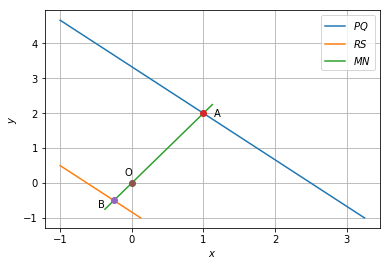
\includegraphics[scale=0.7]{figure.png}
\end{frame}
\end{document}
